
%% bare_jrnl.tex
%% V1.4b
%% 2015/08/26
%% by Michael Shell
%% see http://www.michaelshell.org/
%% fores IEEEtran.cls version 1.8b or later) with an IEEE
%% journar current contact information.
%%
%% This is a skeleton file demonstrating the use of IEEEtran.cls
%% (requil paper.
%%
%% Support sites:
%% http://www.michaelshell.org/tex/ieeetran/
%% http://www.ctan.org/pkg/ieeetran
%% and
%% http://www.ieee.org/

%%*************************************************************************
%% Legal Notice:
%% This code is offered as-is without any warranty either expressed or
%% implied; without even the implied warranty of MERCHANTABILITY or
%% FITNESS FOR A PARTICULAR PURPOSE! 
%% User assumes all risk.
%% In no event shall the IEEE or any contributor to this code be liable for
%% any damages or losses, including, but not limited to, incidental,
%% consequential, or any other damages, resulting from the use or misuse
%% of any information contained here.
%%
%% All comments are the opinions of their respective authors and are not
%% necessarily endorsed by the IEEE.
%%
%% This work is distributed under the LaTeX Project Public License (LPPL)
%% ( http://www.latex-project.org/ ) version 1.3, and may be freely used,
%% distributed and modified. A copy of the LPPL, version 1.3, is included
%% in the base LaTeX documentation of all distributions of LaTeX released
%% 2003/12/01 or later.
%% Retain all contribution notices and credits.
%% ** Modified files should be clearly indicated as such, including  **
%% ** renaming them and changing author support contact information. **
%%*************************************************************************


% *** Authors should verify (and, if needed, correct) their LaTeX system  ***
% *** with the testflow diagnostic prior to trusting their LaTeX platform ***
% *** with production work. The IEEE's font choices and paper sizes can   ***
% *** trigger bugs that do not appear when using other class files.       ***                          ***
% The testflow support page is at:
% http://www.michaelshell.org/tex/testflow/



\documentclass[journal]{IEEEtran}


% correct bad hyphenation here
\hyphenation{op-tical net-works semi-conduc-tor}

\usepackage{graphicx}
\usepackage{caption}
\usepackage{hyperref} 

\begin{document}

\title{INF6600 Rapport TP4 \\ Améliorations au système de contrôle d'un drone fermier}


\author{Daniel~Lussier-Lévesque et Ian~Gagnon}

% make the title area
\maketitle

% As a general rule, do not put math, special symbols or citations
% in the abstract or keywords.
\begin{abstract}
L'implémentation d'un système de contrôle de drone fermier a été réalisé progressivement tout au long de la session en commençant par un module TrueTime avec un système continu déjà implémenté en Simulink. Par la suite, l'implémentation a continué sur une machine virtuelle QNX roulant sous VMware, avec certaines fonctions déjà fournies. Ce rapport se concentre sur ce qui a été fait sur cette base de code pour améliorer les aspects les plus importants. La première étape a été d'implémenter un système de log qui nous permettent de voir comment se comporte l'ordonnancement des tâches et la performance du système. Par la suite, malgré le manque de droits d'accès qui nous permettraient de comprendre l'ensemble des problèmes de performances, nous avons toutefois été capable de les mesurer et de les documenter. Un système graphique vivant en dehors de la machine virtuelle nous permettant de valider le comportement du système a aussi été implémenté.
\end{abstract}


\section{Introduction}
\IEEEPARstart{L}{e} système de contrôle considéré est celui d'un drone autonome capable de se déplacer sur trois axes et ayant une caméra fixe pour prendre en photo l'ensemble d'un champs. Le drone doit naviguer les champs et prendre des photos jusqu'à ce que la mémoire soit pleine, puis transmettre les photos à une station base. Lorsque la batterie est presque vide (10\%), le drone doit retourner à la station base pour être rechargé. 

Le système de contrôle implémente le contrôle de la navigation (où le drone va), le contrôle de la batterie (est-il temps d'aller recharger la batterie?) et le contrôle mission (quelle séquence d'étapes doit être exécutés pour opérer avec succès?).

Le système de contrôle de drone sur lequel nous avons apportés nos modifications est un système simple où la communication entre le système continu et discret est effectué par des variables atomiques et par l'enregistrement de \textit{callbacks}. La communication en dehors du système s'effectue par des messages de log sur la console de debug où à intervalle régulier (chaque seconde) l'état du drone est envoyé. Toutes les tâches sont asynchrones les unes par rapport aux autres et roulent sur leur propre fil d'exécution. Nous avons choisi de mettre à jour le système de contrôle du drone toutes les 100 ms.

De plus, l'implémentation du système de contrôle doit être accompagné d'une plateforme de simulation d'un environnement dans lequel opérer, qui comprend le temps de réponse de la caméra, les variations d'orientation et de vitesses, le temps de transmission de photo à la station base et la charge et décharge de la batterie. Le système continu est mis à jour toutes les 20ms de sorte qu'il soit significativement plus rapide que le système de contrôle. De cette manière, le système discret ne voit pas énormément de différence dépendamment s'il se fait juste avant ou juste après une mise-à-jour du système continu.

L'ensemble des photos prises peut être visualisé à travers une carte du monde qui est mis à jour à chaque transmission et montre quelle région a été prise en photo. La carte doit être accédée en allant chercher les fichiers sur le système de fichier de la machine virtuelle.

La politique d'ordonnancement utilisée est un systèmes de priorités fixes et un ordonnancement FIFO pour chaque niveau de priorité. Le choix a été fait de placer la priorité du contrôle caméra avant celle du contrôleur de navigation parce qu'il est plus facile de compenser pour une échéance manquée dans le cas de la navigation (une photo manquée implique de défaire les dernières mise-à-jour de navigation pour reprendre la photo).

La machine virtuelle roule sous QNX 7.0 sous VMware Workstation avec un hôte Windows 10. La machine hôte à un processeur d'Intel à quatre coeurs, le i7 3770, avec 16 GB de mémoire DDR3 et utilise un Seagate ST1000DM003 comme disque dur. 


% An example of a floating figure using the graphicx package.
% Note that \label must occur AFTER (or within) \caption.
% For figures, \caption should occur after the \includegraphics.
% Note that IEEEtran v1.7 and later has special internal code that
% is designed to preserve the operation of \label within \caption
% even when the captionsoff option is in effect. However, because
% of issues like this, it may be the safest practice to put all your
% \label just after \caption rather than within \caption{}.
%
% Reminder: the "draftcls" or "draftclsnofoot", not "draft", class
% option should be used if it is desired that the figures are to be
% displayed while in draft mode.
%
%\begin{figure}[!t]
%\centering
%\includegraphics[width=2.5in]{myfigure}
% where an .eps filename suffix will be assumed under latex, 
% and a .pdf suffix will be assumed for pdflatex; or what has been declared
% via \DeclareGraphicsExtensions.
%\caption{Simulation results for the network.}
%\label{fig_sim}
%\end{figure}

% Note that the IEEE typically puts floats only at the top, even when this
% results in a large percentage of a column being occupied by floats.


% An example of a double column floating figure using two subfigures.
% (The subfig.sty package must be loaded for this to work.)
% The subfigure \label commands are set within each subfloat command,
% and the \label for the overall figure must come after \caption.
% \hfil is used as a separator to get equal spacing.
% Watch out that the combined width of all the subfigures on a 
% line do not exceed the text width or a line break will occur.
%
%\begin{figure*}[!t]
%\centering
%\subfloat[Case I]{\includegraphics[width=2.5in]{box}%
%\label{fig_first_case}}
%\hfil
%\subfloat[Case II]{\includegraphics[width=2.5in]{box}%
%\label{fig_second_case}}
%\caption{Simulation results for the network.}
%\label{fig_sim}
%\end{figure*}


\section{Lacunes du système de base}
\label{lacunes}

Le système décrit plus haut a plusieurs lacunes importantes. Nous allons ici nous focaliser sur les trois principales faiblesses qui nous ont empêcher de réaliser correctement plusieurs améliorations auxquels nous avions pensés. Il va s'en dire que nous avons penser plus important de régler ces lacunes au meilleur de nos capacités en priorité.

\subsection{Peu de visibilité sur l'état du système}

Le principal problème est qu'avec le système de base, nous ne savons pas si le système est \emph{correct}, c'est à dire que le système effectue les actions que l'ont s'attend à ce qu'il fasse. Les messages de logs qui sont envoyés sont répétitifs et il est facile de manquer un comportement anormal dans les 1800 messages que comportent une séquence d'exécution. De plus, il est impossible de savoir ce qui se passe à l'intérieur de cette période d'une seconde. une période plus courte n'est toutefois pas envisageable: il serait impossible d'analyser l'entièreté du message en temps réel et donc encore plus facile de manquer une information inattendue. Il n'est pas non plus envisageable d'analyser les données à la fin de la simulation: la console de debug ne peut contenir qu'un nombre limité de messages.

En conséquence, il n'est pas possible de qualifier le système d'aucune manière: un problème de comportement du système demanderait une correction importante au code qui invaliderait l'ensemble des mesures effectués. Comme une séance de simulation dure 30 minutes, il serait difficile d'arriver à un ensemble de résultat suffisant dans un temps raisonnables si nos mesures devaient être invalidés. Sans mesures fiables, il est impossible de déterminer si une tentative d'amélioration du système améliore réellement le système. Pour cette raison, cette lacune est considérée comme la plus importante du système implémenté.

\subsection{Aucune visibilité sur la qualité de l'ordonnancement}

En assumant que le comportement du système est correct, nous ne pouvons toujours pas penser à améliorer les performances du système ou rajouter de nouvelles fonctions utiles parce que nous n'avons aucune métrique de performance de disponible. Nous ne savons pas si les tâches manquent leur échéance de manière régulière et arrivent tout juste à rester fonctionnels, ou au contraire si il y a largement de ressources disponibles pour de nouvelles tâches.

Dans le cas où le comportement du système n'est pas celui attendu, les métriques de qualité d'exécution nous sont aussi utile pour comprendre les problèmes. Si une tâche est en famine parce que les tâches plus prioritaires prennent toutes les ressources, ce sera facilement visible et évitera une longue séance de debug en aveugle. Nous considérons cette lacune comme fondamentale et bloquante pour des améliorations à d'autres aspect du système.

\subsection{Pics de latence}

Après avoir apportés les modifications qui seront détaillés à la section \ref{ameliorations}, nous avons réalisés que le système tel que simulé avait encore une lacune qui bloquait des améliorations que nous avions planifiés: le système est affecté par des pics de latences non-déterministes. Ces pics de latences affectent toutes les tâches en même temps. Plus spécifiquement, ils affectent des tâches qui n'acquirent pas de mutex où autre verrou global et communiquent uniquement par des variables atomiques. On peut donc conclure que ces pics arrivent au niveau système et non au niveau de l'ordonnancement ou au niveau de la communication. 

En plus d'affecter les performances du systèmes et de le rendre moins fiable, un impact important de ces pics de latences est que toutes les métriques de pire temps d'exécution ou de déviations standard sont affectés de manière aléatoire et qu'une comparaison avant et après d'une tentative d'amélioration est noyée dans le bruit de ces pics.

Les pics des latences durent plusieurs millisecondes. Plusieurs tentatives de contourner le problème ont été essayé: réduire le nombre de cœurs du système de contrôle, augmenter le nombre de cœurs du système et déplacer la machine virtuelle du disque réseau au disque dur local. Déplacer la machine virtuelle à permis de réduire significativement la durée de ces pics, mais aucune des ces tentatives n'a permis de ramener les variations de latences à des temps raisonnables.

\section{Améliorations apportées}\label{ameliorations}
\begin{figure}
	\centering
	\captionsetup{justification=centering}
	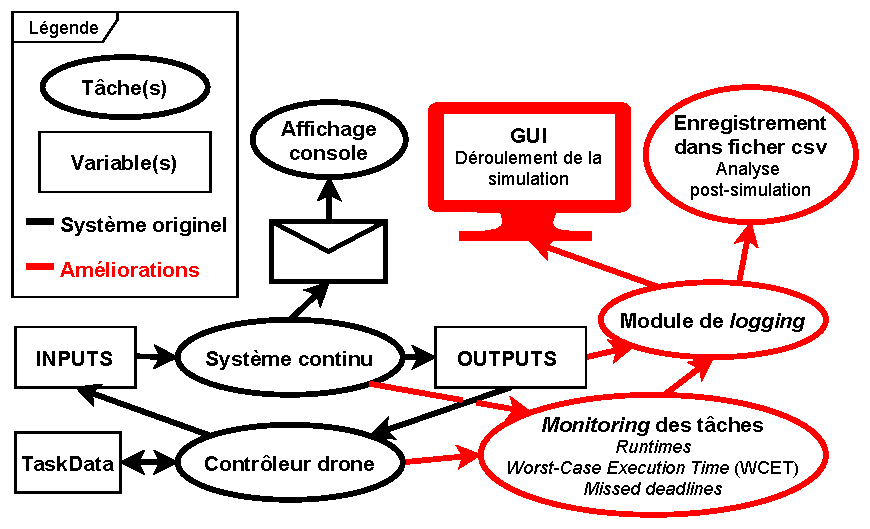
\includegraphics[width=\linewidth]{diagrammeDeTaches_Simple.pdf}
	\caption{Diagramme de tâches du système}
	\label{taskDiagram}
\end{figure}

Des lacunes présentées à la section précédente, les deux premières concernant la visibilité du système ont été identifiées comme prioritaires. 
Pour y remédier, des améliorations sont proposées et illustrées à la Figure \ref{taskDiagram}. Un \textit{monitoring} des tâches récolte d'abord les métriques d'exécution pour chaque tâche, un module de \textit{logging} sert ensuite à regrouper les informations pour finalement les enregistrer en format csv. En supplément, un \textit{Graphical User Interface} (GUI) permet de suivre le déroulement de la simulation.

\subsection{Monitoring des tâches}

Pour chaque tâche qui s'exécute, le temps d'exécution est calculé en faisant la différence entre les temps initial et final obtenus par la fonction \verb|std::chrono::steady_clock::now()| et stockés dans des variables atomiques. Ainsi, la durée de la dernière exécution (\textit{last runtime}), le pire cas (WCET pour \textit{Worst-Case Execution Time}) et les échéances manquées (\textit{missed deadlines}) sont comptabilisés. Notons, que l'horloge du système, avec sa granularité d'une milliseconde, limite la précision des données.

\subsection{Logging}

Une fois que nous avons implanté le code pour avoir l'information dans des variables, il faut penser à un moyen de la communiquer. Il a donc fallu implémenter une nouvelle fonction (avec le code de \textit{monitoring} associé) pour lire l'ensemble des variable et les transmettre vers les nouvelles sorties. Nous avons décider d'exécuter la tâche toutes les 100 millisecondes afin de ne pas surcharger le système. Cette fonction est appelée par la tâche de \textit{monitoring} déjà existante qui auparavant ne poussait les donnée que vers la console une fois toute les secondes.

\subsection{Sortie en fichier csv}

La sortie qui permet de faire une analyse compréhensive du système est un simple fichier csv qui est sauvegardé en mémoire non-volatile au fur et à mesure que la simulation avance. Le format csv étant supporté par pratiquement tous les outils d'analyse et de base de données, il est donc facile de s'en servir pour obtenir des statistiques sur un grand nombre d'exécutions pour ensuite les formater adéquatement en tableaux, en graphiques ou en générant un rapport (e.g. en JSON). En effet, que ce soit à l'aide de scripts (avec Python, R ou MATLAB) ou manuellement (avec Microsoft Excel ou LibreOffice Calc), l'analyse sera infiniment plus poussée que celle obtenue avec la sortie en console. De plus, cette approche permet d'étudier en détails les circonstances d'un \textit{crash}.
 
\subsection{GUI}
Un GUI a été implémenté en Python afin de suivre l'avancement de la simulation. Comme il s'agit d'une preuve de concept et que le focus de ce projet est l'implémentation sous QNX, l'interface graphique est limitée à un strict minimum (voir section~\nameref{resultats}). L'accent est plutôt mis sur le transfert de données. À cet égard, l'hypothèse (très réaliste) que le drone transmet ces images à la base via une connexion réseau est émise et cette connexion est exploitée pour établir la communication avec le GUI en utilisant un \textit{socket} internet avec le protocole TCP/IP. Comme il n'y a pas de \textit{End Of Transmission} (EOT) sur un \textit{socket}, une convention doit être choisie afin d'assurer un bon transfert de données: message d'une longueur fixe, message délimité (i.e. avec caractères spéciaux de début et fin) ou  message avec une entête indiquant sa longueur. Ici, pour garder le tout le plus simple possible, la longueur des paquets est fixée et des caractères de remplissage (i.e. des espaces) sont ajoutés à la fin des trames de données pour ajuster la taille des paquets. De plus, un délai sur la connexion, une gestion de déconnexion ainsi qu'un avertissement de fin de simulation sont ajoutés pour prévenir les erreurs et éviter les \textit{deadlocks}.

\section{Résultats}\label{resultats}

\subsection{Analyse du système}
Avant d'analyser le système en détails à l'aide du fichier csv fournit par nos améliorations, la fonctionnalité de l'implémentation de base est validée à la l'aide de l'image en sortie de la simulation générée par la fonction \textit{transmitPhotos()}. L'image agrandie (Figure \ref{fig:farmMap}) démontre effectivement que l'intégralité du champ 22, soit le champ balayé lors de la simulation, a été photographié.

\begin{figure}
	\centering
	\captionsetup{justification=centering}
	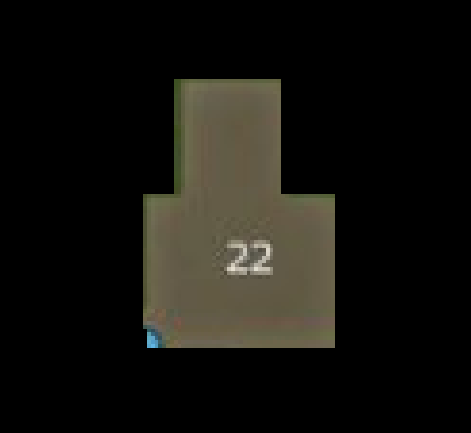
\includegraphics[width=1.8in]{farmMap.png}
	\caption{Image agrandie de la zone couverte par le drone}
	\label{fig:farmMap}
\end{figure}


\#TODO Parler des vrais résultats et mettre les graphiques


\subsection{Description du GUI}
\begin{figure}
	\centering
	\captionsetup{justification=centering}
	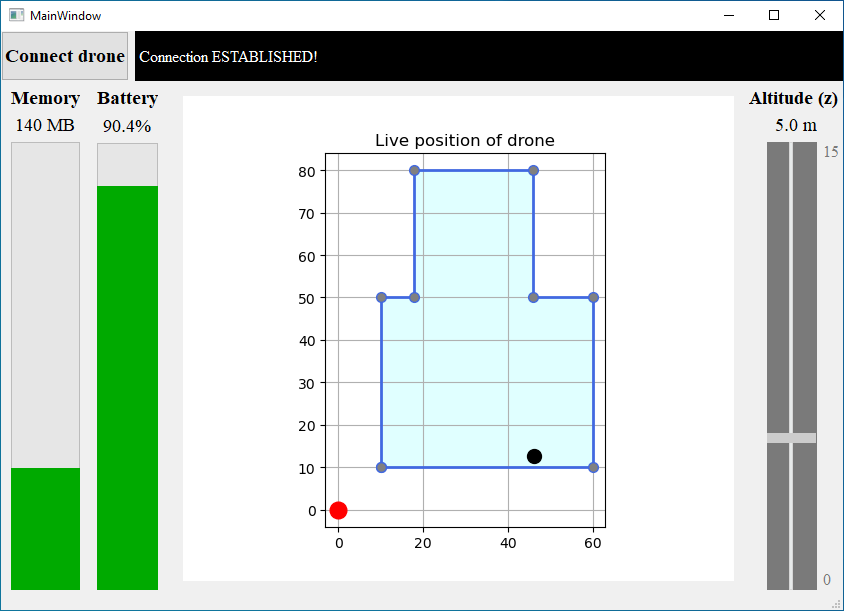
\includegraphics[width=\linewidth]{GUI_image.png}
	\caption{GUI durant la simulation}
	\label{fig:GUI}
\end{figure}

Dans la communication TCP/IP, le serveur roule sur QNX et le client sur le GUI. Après avoir ouvert le GUI, il faut donc d'abord lancer la simulation QNX (qui va partir le serveur) et ensuite appuyer sur le bouton "Connect drone" pour établir la connexion. Le GUI, présenté à la Figure \ref{fig:GUI}, affiche les paramètres de base de la simulation, soit: la mémoire, le niveau de batterie, la position du drone (x, y) et son altitude (z). De plus, une vidéo montrant le GUI en fonction (i.e. la simulation en accélérée) est disponible au lien suivant: \href{https://drive.google.com/file/d/1W9yt0Z4YxCwr0TjXkgv12WVO9TSmWGtv/view?usp=sharing}{INF6600-GUI-DEMO}.


\section{Conclusion}
Dans cet article, nous avons décrit les améliorations apportées à l'implémentation d'un système de contrôle de drone fermier. L'analyse du système de base a soulevé des lacunes importantes en ce qui concerne les visibilités de l'état du système et de la qualité de l'ordonnancement. En effet, ce manque d'informations rend l'analyse du système et de ses performances laborieuse pour ne pas dire impossible. 

Afin de pallier à ce manque de données, nous avons dans un premier temps implémenté un \textit{monitoring} des tâches avec un module de \textit{logging} permettant de recueillir de précieuses informations et de les enregistrer pour les analyser ultérieurement. Cela nous a permis d'étudier le système et de réaliser que...

\#TODO Parler brièvement des conclusions de l'analyse

Dans un second temps, nous avons ajouté un GUI communiquant avec le drone via une connexion réseau utilisant le protocole TCP/IP. Ce dernier affiche l'état du système durant la simulation et aide l'utilisateur à repérer un comportement inattendu du drone. Dans l'optique d'un déploiement réel du système sur une ferme, cette interface graphique roulant au niveau de la base (vraisemblablement la maison du fermier) s'avérerait utile puisqu'elle permettrait au fermier du suivre le drone lors de sa mission et de réagir en cas de problèmes.

\vspace{2mm}

Cependant, les améliorations apportées ont des limites...


\vspace{2mm}
Il y a plusieurs directions pour les travaux futurs. Premièrement, il serait intéressant d'analyser les performances du système en utilisant plus de \textit{cores} (8 par exemple). Une telle parallélisation des tâches, si bien réalisée, pourrait considérablement augmenter la rapidité du système.

Deuxièmement, la sécurité du système pourrait être rehaussée par l'utilisation de partitions. En isolant les processus de cette manière, on éviterait que la défaillance d'une tâche fasse planter tout le système. Par exemple, une erreur du système de communication n'aurait aucun impact sur le système de navigation, ce qui n'est pas une certitude présentement.

Dernièrement, d'un point de vue sécurité pour une utilisation réelle du système, il serait pertinent d'ajouter un bouton d'urgence à l'interface graphique pour arrêter le drone de force ou le ramener immédiatement à la base dans le cas où l'algorithme de contrôle aurait un raté (e.g. un mauvais calcul qui enverrait le drone à 1000 m d'altitude). 







% if have a single appendix:
%\appendix[Proof of the Zonklar Equations]
% or
%\appendix  % for no appendix heading
% do not use \section anymore after \appendix, only \section*
% is possibly needed

% use appendices with more than one appendix
% then use \section to start each appendix
% you must declare a \section before using any
% \subsection or using \label (\appendices by itself
% starts a section numbered zero.)
%

% references section

% can use a bibliography generated by BibTeX as a .bbl file
% BibTeX documentation can be easily obtained at:
% http://mirror.ctan.org/biblio/bibtex/contrib/doc/
% The IEEEtran BibTeX style support page is at:
% http://www.michaelshell.org/tex/ieeetran/bibtex/
%\bibliographystyle{IEEEtran}
% argument is your BibTeX string definitions and bibliography database(s)
%\bibliography{IEEEabrv,../bib/paper}
%
% <OR> manually copy in the resultant .bbl file
% set second argument of \begin to the number of references
% (used to reserve space for the reference number labels box)
\begin{thebibliography}{1}

\bibitem{IEEEhowto:kopka}
H.~Kopka and P.~W. Daly, \emph{A Guide to \LaTeX}, 3rd~ed.\hskip 1em plus
  0.5em minus 0.4em\relax Harlow, England: Addison-Wesley, 1999.

\end{thebibliography}




% Can be used to pull up biographies so that the bottom of the last one
% is flush with the other column.
%\enlargethispage{-5in}



% that's all folks
\end{document}


